\newpage
\section{Materiais e métodos}

Os experimentos realizados nessa prática foram embasados no Princípio de Arquimedes, o qual afirma que um fluido exerce uma força ascendente em um corpo que se encontra mergulhado no mesmo fluido, sendo que o módulo dessa força corresponde ao peso do volume do líquido deslocado.

Assim, foi montado um dispositivo dentro do laboratório para verificar tal princípio, de modo que um pequeno cilindro fosse acoplado na extremidade inferior de uma mola posicionada verticalmente. Logo, quando o cilindro foi solto, seu peso (força gravitacional) deformou a mola até tal força se igualar com a força elástica proporcionada em função do tempo, enquanto uma régua posicionada verticalmente próximo à mola viabilizou a marcação da deformação.

\begin{figure}[H]
    \centering
    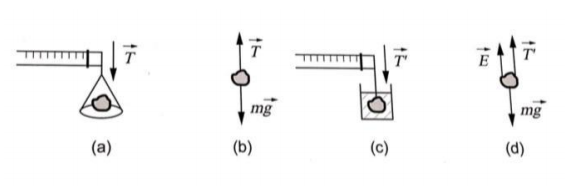
\includegraphics[scale=0.8]{images/Experimento1.png}
    \caption{Esquema de Forças atuando em uma balança de tração.}
\end{figure}

Dois casos foram realizados. O primeiro foi com o cilindro, sem submersão deste em um líquido, foi solto, enquanto o segundo houve submersão do corpo cilíndrico em um recipiente com água após ser solto.

% =============== EXPERIMENTO 2 ===================== %

\subsection{Determinação do volume e da densidade de um sólido com
uma balança}

Maia


% =============== EXPERIMENTO 3 ===================== %

\subsection{Determinação do volume e da densidade de um sólido
utilizando um Areômetro de Nicholson}

Para essa prática vamos utilizar um Areômetro de Nicholson, que é formado por um cilindro oco de metal, ao qual estão presos dois pratos: um na parte de cima do cilindro, e outro na parte de baixo, como mostrado na figura a seguir.\\

\begin{figure}[H]
    \centering
    \includegraphics[scale=1.0]{images/Areômetro 1.png}
    \caption{Representação da estrutura de um Areômetro de Nicholson}
\end{figure}

O volume de areômetro será denominado $V_{ar}$ e seu peso total $P_{ar}$.\\

Uma haste o cilindro ao prato superior conta com uma marcação que referencia a medida, e é chamada de "traço de afloramento". O "afloramento" é obtido quando o aparato se encontra submerso em um líquido, em equilíbrio hidrostático, com o "traço de afloramento" coincidindo com o nível do fluido.\\

\begin{figure}[H]
    \centering
    \includegraphics[scale=1.0]{images/Areômetro 2.png}
    \caption{Representação do experimento para determinar o volume de um sólido utilizando um areômetro}
\end{figure}

Após termos entendido do que é constituído o Areômetro de Nicholson, vamos utilizá-lo para calcular o volume - e consequentemente - a densidade de um sólido desconhecido.

Para o cálculo do volume do sólido, primeiramente precisamos determinar a massa dele $m_s$, com a ajuda de uma balança digital. Colocamos então, o sólido no prato superior do areômetro e vamos adicionando uma massa $m_a$ até que o "afloramento" seja atingido - por conta do equilíbrio hidrostático em água. Mediremos a massa adicionada $m_a$, e anotaremos o valor. 
Dessa forma, a equação do equilíbrio hidrostático é:

\[ (m_s + m_a)g + P_{ar} = \rho _{agua} g V_{ar} \]

Então retiramos o sólido do prato superior, e o colocamos no prato inferior (que ficará submerso). Agora, adicionaremos uma massa $m_a'$ no prato superior até que ocorra o "afloramento". O equilíbrio hidrostático nos dá uma nova equação:

\[ (m_s + m_a')g + P_{ar} = \rho _{agua} g (V_{ar} + V_s) \]

Vamos combinar as duas equações acima, para obter o volume do sólido e sua densidade:

\[ V_s = \frac{(m_a' - m_a)}{\rho _{agua}} \]

e

\[ \rho _s = \frac{m_s}{V_s} = \frac{m_s}{(m_a' - m_a)} \rho _{agua} \]\\

Podemos dizer que a força de empuxo sobre o sólido é basicamente a diferença entre os pesos necessários para que ocorra o "afloramento" com o sólido no prato de cima ou no prato de baixo, pois quando ele está dentro do líquido, o empuxo sobre ele demanda uma massa $m_a'$ maior para compensá-lo. \\


 



% =============== EXPERIMENTO 4 ===================== %

\subsection{Determinação da densidade de um líquido utilizando o
Areômetro de Nicholson}

Da mesma forma que o experimento anterior, utilizaremos o areômetro como instrumento para determinar a densidade, mas agora não de um sólido, mas sim de um líquido. Ele não foi feito inventado para essa finalidade, mas produz ainda sim um resultado aceitável.

\begin{figure}[H]
    \centering
    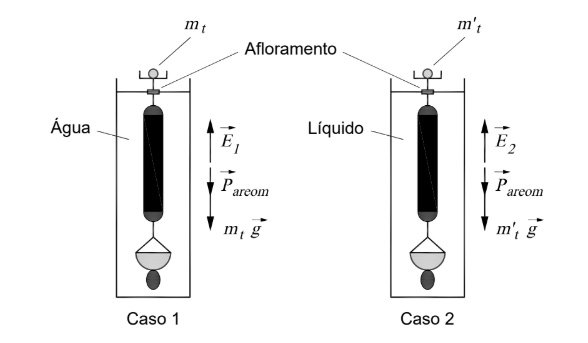
\includegraphics[scale=0.8]{images/aerometro-densidade-liquido.png}
    \caption{Representação do experimento para determinar a densidade de um líquido utilizando um areômetro}
\end{figure}

Para começar, iremos inserir o instrumento numa líquido cujo valor de $\rho$ é conhecido (no caso será água a 25°C). Então colocamos o recipiente com água e taramos a balança, para que agora possamos aflorar o areômetro, anotando o valor da massa do areômetro junto com os pesinhos ($m_{ar} + m_{pa}$). Pesando depois as massinhas separadamente ($m_t$) podemos determinar o valor do volume do areômetro, que será dado fórmula básica da densidade:

\[ V_{ar} = \frac{m_{ar} + m_t}{\rho _{agua}} \]

\[ \delta V_{ar} = \frac{\delta m_{ar} + \delta m_t}{\rho _{agua}} \]

Com esse dado em mão podemos partir para a determinação da densidade do líquido desconhecido. Assim sendo, iremos primeiramente encher a proveta com esse líquido e aflorar o areômetro lá imerso, e pesaremos o valor das massinhas utilizadas ($m_t'$). Com esse valor em mãos, podemos utilizar a fórmula deduzida no vídeo para o cálculo de densidades utilizando um aerômetro:

\[ \rho _x = \rho _{agua} + \frac{m_t' - m_t}{V_{ar}} \]

\[ \delta \rho _x = \rho _{agua} \cdot \frac{(\delta m_t' + \delta m_t) \cdot V_{ar} + \delta V_{ar} \cdot (m_t' - m_t)}{V_{ar}^2} \]

Após a obtenção de $\rho _x$ vamos procurar online tabelas com valores para comparar o nosso resultado.

